\documentclass[UTF8]{beamer}
\usepackage{ctex}
\usepackage{hyperref} %用于设置 PDF 的信息
\usepackage{setspace} %用于设置行间距
\usepackage{listings} %用于代码高亮
\usepackage{xcolor} %用于处理颜色
\usepackage{ulem} %用于各种线
\usepackage{amsmath} %用于数学公式(如 \begin{align})
\usepackage{booktabs} %用于表格画线
\usepackage{graphicx} %用于插入图片
%\usepackage[top = 1.0in, bottom = 1.0in, left = 1.0in, right = 1.0in]{geometry} %设置页边距

\hypersetup{
	pdfauthor={Orange}
}

\usetheme[secheader]{Madrid}

\title{数论函数基础(入门)}
\author{Orange}
\institute{CQ No.11 High}
\date{\today}

\begin{document}
	\heiti

	\begin{frame}
		\titlepage
	\end{frame}

	\section{零碎的东西}
	\begin{frame}
		\frametitle{\insertsection}
		把定义域为正整数,值域被包含于复数域的函数称为数论函数。

		\pause
		\bigskip
		将真或假的命题 放在方括号中。当命题 为真时,命题的结果为 1;
		为假时,结果为 0。这种表示方法叫作艾弗森约定。

		$$
		[\mathrm{statement}~k] =
		\left\{
		\begin{matrix}
		0, & k = false
		\\
		1, & k = true
		\end{matrix}
		\right.
		$$
	\end{frame}

	\section{积性函数}
	\subsection{唯一分解定理}
	\begin{frame}
		\frametitle{\insertsubsection}
	\end{frame}

	\subsection{积性函数与完全积性函数}
	\begin{frame}
		\frametitle{\insertsubsection}
	\end{frame}

	\subsection{常见积性函数}
	\subsubsection{奇怪的积性函数}
	\begin{frame}
		\frametitle{\insertsubsection}
		\begin{gather*}
			\epsilon(n) = [n = 1]
			\\
			\mathrm{1}(n) = 1
			\\
			\mathrm{id}(n) = n
		\end{gather*}
	\end{frame}

	\subsubsection{正常的积性函数}
	\begin{frame}
		\frametitle{\insertsubsection}
		\begin{gather*}
			\varphi(n) = \sum _{i = 1} ^{n} [\gcd(i, n) = 1]
			\\
			\sigma_k(n) = \sum _{d \mid n} d^k
		\end{gather*}
	\end{frame}

	\subsection{欧拉筛}
	\subsubsection{代码}
	\begin{frame}
		\frametitle{\insertsubsection}
	\end{frame}

	\subsubsection{时间复杂度}
	\begin{frame}
		\frametitle{\insertsubsubsection}
	\end{frame}

	\subsubsection{使用欧拉筛求积性函数}
	\begin{frame}
		\frametitle{\insertsubsubsection}
	\end{frame}

	\subsection{e.g. (有可能有用的一个子问题)}
	\begin{frame}
		\frametitle{\insertsubsection}
		给定一个正整数 $k$,有很多组询问,
		每次询问给定一个正整数 $n(n \le 10^7)$,求:

		$$
		\sum_{i = 1}^{n} i^k
		$$

		结果对 $998244353$ 取模。
	\end{frame}

	\subsection{e.g. 1306. GCD 1}
	\begin{frame}
		\frametitle{\insertsubsection}
		给定一个正整数 $n(n \le 10^7)$,
		求满足 $1 \le x, y \le n$ 且 $\gcd(x, y)$ 为素数的数对 $(x, y)$ 有多少对。
	\end{frame}

	\section{狄利克雷卷积}
	\begin{frame}
		\frametitle{\insertsection}
		定义数论函数 h:

		$$
		h(n) = (f * g)(n) = \sum_{d \mid n} f(d)g(\frac {n} {d})
		$$

		称 $h$ 为 $f$ 和 $g$ 狄利克雷(Dirichlet)卷积。

		\pause
		\bigskip
		狄利克雷卷积满足:

		$$
		f * g = g * f
		$$
		$$
		f * g * h = f * (g * h)
		$$
		$$
		f * \epsilon = f
		$$
	\end{frame}

	\subsection{积性}
	\begin{frame}
		\frametitle{\insertsubsection}
		如果 $f$ 和 $g$ 均为积性函数,则有 $f * g$ 为积性函数。

		\pause
		\sout{如果 $f$ 和 $g$ 均为完全积性函数,则有 $f * g$ 为完全积性函数。}

		\pause
		\bigskip
		所以积性函数的狄利克雷卷积可以使用欧拉筛计算。
	\end{frame}
	
	\subsection{e.g. Longge's problem}
	\begin{frame}
		\frametitle{\insertsubsection}
		给定 unsigned int 范围内的正整数 $n$,计算:

		$$
		\sum_{i = 1}^{n} \gcd(i, n)
		$$
	\end{frame}

	\begin{frame}
		\begin{figure}[ht]
		\centering
		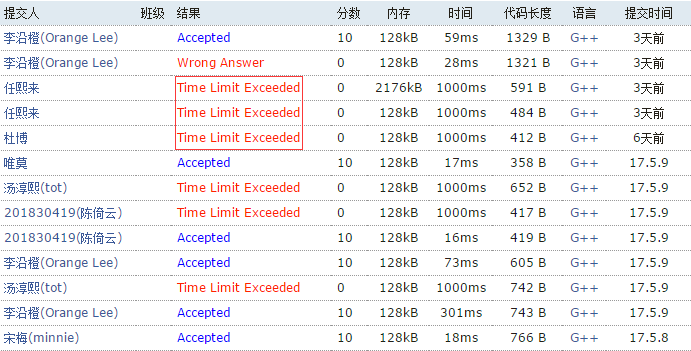
\includegraphics[scale=0.4]{pic/1.png}
		\end{figure}

		\begin{center}
			TLE 的同学,请复习一下时间复杂度。
		\end{center}
	\end{frame}

	\subsection{e.g. 1311. GCD 6}
	\begin{frame}
		\frametitle{\insertsubsection}
		其中的一个子问题。

		\bigskip
		计算:
		$$
		\sum_{n = 1}^{10^7}
		\sum_{d \mid n} d \cdot \varphi(d)
		$$
	\end{frame}

\end{document}\frametitle{\insertsubsection}